\section{First Results}

In this Section, we\textquotesingle ll briefly discuss the dynamics of the equation (\ref{eq:EquationOfMotion}), with mostly numerical results. 

The dipole\textquotesingle s dynamics was studied for small amplitude of oscillation of the magnetic field. We used two main values for the parameter $\varepsilon$, $\varepsilon = 0.05$ and $\varepsilon = 0.5$, and the following initial conditions for both cases:
\begin{equation}
    \begin{cases}
        \theta (0) &= 1\\        
        \dot{\theta}(0) &= 0
    \end{cases}
\end{equation} 
In the former case, $\varepsilon = 0.05$, we verify that the dipole\textquotesingle s movement was periodic for all the values of the frequency of the magnetic field $\Omega$ in $[-3,3]$, and as expected, the dipole behaved like a simple pendulum. 

However, for the latter case, $\varepsilon = 0.5$, the dipole\textquotesingle s movement was much more complex. For some subintervals in the frequency range in $[-3,3]$, the movement was not periodic, figure \ref{fig:omega075}, and maybe not even limited. 

In the cases where the movement was oscillatory, the oscillation frequency was not comparable to the frequency of the magnetic field, and for the most time, the frequency of the movement was the natural frequency of the system. 

\begin{figure}
    \centering
    \scalebox{0.7}{% GNUPLOT: LaTeX picture with Postscript
\begingroup
  \makeatletter
  \providecommand\color[2][]{%
    \GenericError{(gnuplot) \space\space\space\@spaces}{%
      Package color not loaded in conjunction with
      terminal option `colourtext'%
    }{See the gnuplot documentation for explanation.%
    }{Either use 'blacktext' in gnuplot or load the package
      color.sty in LaTeX.}%
    \renewcommand\color[2][]{}%
  }%
  \providecommand\includegraphics[2][]{%
    \GenericError{(gnuplot) \space\space\space\@spaces}{%
      Package graphicx or graphics not loaded%
    }{See the gnuplot documentation for explanation.%
    }{The gnuplot epslatex terminal needs graphicx.sty or graphics.sty.}%
    \renewcommand\includegraphics[2][]{}%
  }%
  \providecommand\rotatebox[2]{#2}%
  \@ifundefined{ifGPcolor}{%
    \newif\ifGPcolor
    \GPcolortrue
  }{}%
  \@ifundefined{ifGPblacktext}{%
    \newif\ifGPblacktext
    \GPblacktexttrue
  }{}%
  % define a \g@addto@macro without @ in the name:
  \let\gplgaddtomacro\g@addto@macro
  % define empty templates for all commands taking text:
  \gdef\gplbacktext{}%
  \gdef\gplfronttext{}%
  \makeatother
  \ifGPblacktext
    % no textcolor at all
    \def\colorrgb#1{}%
    \def\colorgray#1{}%
  \else
    % gray or color?
    \ifGPcolor
      \def\colorrgb#1{\color[rgb]{#1}}%
      \def\colorgray#1{\color[gray]{#1}}%
      \expandafter\def\csname LTw\endcsname{\color{white}}%
      \expandafter\def\csname LTb\endcsname{\color{black}}%
      \expandafter\def\csname LTa\endcsname{\color{black}}%
      \expandafter\def\csname LT0\endcsname{\color[rgb]{1,0,0}}%
      \expandafter\def\csname LT1\endcsname{\color[rgb]{0,1,0}}%
      \expandafter\def\csname LT2\endcsname{\color[rgb]{0,0,1}}%
      \expandafter\def\csname LT3\endcsname{\color[rgb]{1,0,1}}%
      \expandafter\def\csname LT4\endcsname{\color[rgb]{0,1,1}}%
      \expandafter\def\csname LT5\endcsname{\color[rgb]{1,1,0}}%
      \expandafter\def\csname LT6\endcsname{\color[rgb]{0,0,0}}%
      \expandafter\def\csname LT7\endcsname{\color[rgb]{1,0.3,0}}%
      \expandafter\def\csname LT8\endcsname{\color[rgb]{0.5,0.5,0.5}}%
    \else
      % gray
      \def\colorrgb#1{\color{black}}%
      \def\colorgray#1{\color[gray]{#1}}%
      \expandafter\def\csname LTw\endcsname{\color{white}}%
      \expandafter\def\csname LTb\endcsname{\color{black}}%
      \expandafter\def\csname LTa\endcsname{\color{black}}%
      \expandafter\def\csname LT0\endcsname{\color{black}}%
      \expandafter\def\csname LT1\endcsname{\color{black}}%
      \expandafter\def\csname LT2\endcsname{\color{black}}%
      \expandafter\def\csname LT3\endcsname{\color{black}}%
      \expandafter\def\csname LT4\endcsname{\color{black}}%
      \expandafter\def\csname LT5\endcsname{\color{black}}%
      \expandafter\def\csname LT6\endcsname{\color{black}}%
      \expandafter\def\csname LT7\endcsname{\color{black}}%
      \expandafter\def\csname LT8\endcsname{\color{black}}%
    \fi
  \fi
    \setlength{\unitlength}{0.0500bp}%
    \ifx\gptboxheight\undefined%
      \newlength{\gptboxheight}%
      \newlength{\gptboxwidth}%
      \newsavebox{\gptboxtext}%
    \fi%
    \setlength{\fboxrule}{0.5pt}%
    \setlength{\fboxsep}{1pt}%
    \definecolor{tbcol}{rgb}{1,1,1}%
\begin{picture}(6480.00,4320.00)%
    \gplgaddtomacro\gplbacktext{%
      \csname LTb\endcsname%%
      \put(726,440){\makebox(0,0)[r]{\strut{}$-1$}}%
      \put(726,806){\makebox(0,0)[r]{\strut{}$-0.8$}}%
      \put(726,1172){\makebox(0,0)[r]{\strut{}$-0.6$}}%
      \put(726,1538){\makebox(0,0)[r]{\strut{}$-0.4$}}%
      \put(726,1904){\makebox(0,0)[r]{\strut{}$-0.2$}}%
      \put(726,2270){\makebox(0,0)[r]{\strut{}$0$}}%
      \put(726,2635){\makebox(0,0)[r]{\strut{}$0.2$}}%
      \put(726,3001){\makebox(0,0)[r]{\strut{}$0.4$}}%
      \put(726,3367){\makebox(0,0)[r]{\strut{}$0.6$}}%
      \put(726,3733){\makebox(0,0)[r]{\strut{}$0.8$}}%
      \put(726,4099){\makebox(0,0)[r]{\strut{}$1$}}%
      \put(858,220){\makebox(0,0){\strut{}$-3$}}%
      \put(1729,220){\makebox(0,0){\strut{}$-2$}}%
      \put(2600,220){\makebox(0,0){\strut{}$-1$}}%
      \put(3471,220){\makebox(0,0){\strut{}$0$}}%
      \put(4341,220){\makebox(0,0){\strut{}$1$}}%
      \put(5212,220){\makebox(0,0){\strut{}$2$}}%
      \put(6083,220){\makebox(0,0){\strut{}$3$}}%
    }%
    \gplgaddtomacro\gplfronttext{%
    \csname LTb\endcsname%%
    \put(152,2270){\rotatebox{-270}{\makebox(0,0){\strut{}$\omega $}}}%
    \put(3471,-112){\makebox(0,0){\strut{}$\Omega$}}%
  }%
    \gplbacktext
    \put(0,0){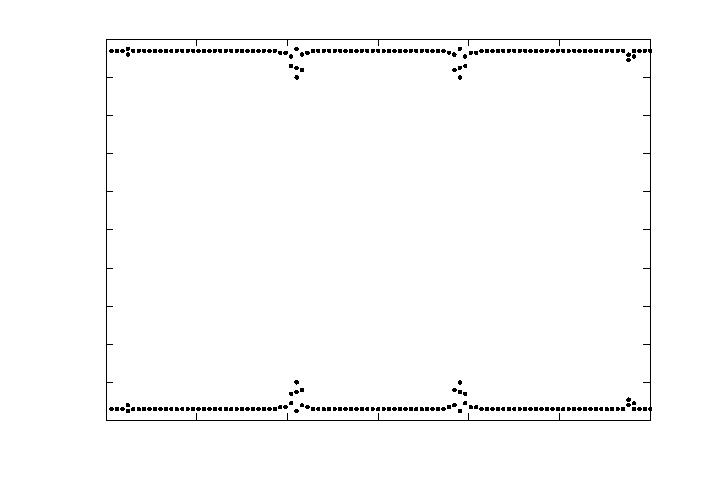
\includegraphics[width={324.00bp},height={216.00bp}]{images/FrequencyBifurcation005}}%
    \gplfronttext
  \end{picture}%
\endgroup
}
    \caption{Bifurcation diagram of frequencies from the oscillating magnetic field $\Omega$ and the response frequencies on the dipole $\omega$, for the case with $\varepsilon = 0.05$.}
    \label{fig:bif005}
\end{figure}

\begin{figure}
    \centering
    \scalebox{0.7}{% GNUPLOT: LaTeX picture with Postscript
\begingroup
  \makeatletter
  \providecommand\color[2][]{%
    \GenericError{(gnuplot) \space\space\space\@spaces}{%
      Package color not loaded in conjunction with
      terminal option `colourtext'%
    }{See the gnuplot documentation for explanation.%
    }{Either use 'blacktext' in gnuplot or load the package
      color.sty in LaTeX.}%
    \renewcommand\color[2][]{}%
  }%
  \providecommand\includegraphics[2][]{%
    \GenericError{(gnuplot) \space\space\space\@spaces}{%
      Package graphicx or graphics not loaded%
    }{See the gnuplot documentation for explanation.%
    }{The gnuplot epslatex terminal needs graphicx.sty or graphics.sty.}%
    \renewcommand\includegraphics[2][]{}%
  }%
  \providecommand\rotatebox[2]{#2}%
  \@ifundefined{ifGPcolor}{%
    \newif\ifGPcolor
    \GPcolortrue
  }{}%
  \@ifundefined{ifGPblacktext}{%
    \newif\ifGPblacktext
    \GPblacktexttrue
  }{}%
  % define a \g@addto@macro without @ in the name:
  \let\gplgaddtomacro\g@addto@macro
  % define empty templates for all commands taking text:
  \gdef\gplbacktext{}%
  \gdef\gplfronttext{}%
  \makeatother
  \ifGPblacktext
    % no textcolor at all
    \def\colorrgb#1{}%
    \def\colorgray#1{}%
  \else
    % gray or color?
    \ifGPcolor
      \def\colorrgb#1{\color[rgb]{#1}}%
      \def\colorgray#1{\color[gray]{#1}}%
      \expandafter\def\csname LTw\endcsname{\color{white}}%
      \expandafter\def\csname LTb\endcsname{\color{black}}%
      \expandafter\def\csname LTa\endcsname{\color{black}}%
      \expandafter\def\csname LT0\endcsname{\color[rgb]{1,0,0}}%
      \expandafter\def\csname LT1\endcsname{\color[rgb]{0,1,0}}%
      \expandafter\def\csname LT2\endcsname{\color[rgb]{0,0,1}}%
      \expandafter\def\csname LT3\endcsname{\color[rgb]{1,0,1}}%
      \expandafter\def\csname LT4\endcsname{\color[rgb]{0,1,1}}%
      \expandafter\def\csname LT5\endcsname{\color[rgb]{1,1,0}}%
      \expandafter\def\csname LT6\endcsname{\color[rgb]{0,0,0}}%
      \expandafter\def\csname LT7\endcsname{\color[rgb]{1,0.3,0}}%
      \expandafter\def\csname LT8\endcsname{\color[rgb]{0.5,0.5,0.5}}%
    \else
      % gray
      \def\colorrgb#1{\color{black}}%
      \def\colorgray#1{\color[gray]{#1}}%
      \expandafter\def\csname LTw\endcsname{\color{white}}%
      \expandafter\def\csname LTb\endcsname{\color{black}}%
      \expandafter\def\csname LTa\endcsname{\color{black}}%
      \expandafter\def\csname LT0\endcsname{\color{black}}%
      \expandafter\def\csname LT1\endcsname{\color{black}}%
      \expandafter\def\csname LT2\endcsname{\color{black}}%
      \expandafter\def\csname LT3\endcsname{\color{black}}%
      \expandafter\def\csname LT4\endcsname{\color{black}}%
      \expandafter\def\csname LT5\endcsname{\color{black}}%
      \expandafter\def\csname LT6\endcsname{\color{black}}%
      \expandafter\def\csname LT7\endcsname{\color{black}}%
      \expandafter\def\csname LT8\endcsname{\color{black}}%
    \fi
  \fi
    \setlength{\unitlength}{0.0500bp}%
    \ifx\gptboxheight\undefined%
      \newlength{\gptboxheight}%
      \newlength{\gptboxwidth}%
      \newsavebox{\gptboxtext}%
    \fi%
    \setlength{\fboxrule}{0.5pt}%
    \setlength{\fboxsep}{1pt}%
    \definecolor{tbcol}{rgb}{1,1,1}%
\begin{picture}(6480.00,4320.00)%
    \gplgaddtomacro\gplbacktext{%
      \csname LTb\endcsname%%
      \put(726,440){\makebox(0,0)[r]{\strut{}$-1$}}%
      \put(726,806){\makebox(0,0)[r]{\strut{}$-0.8$}}%
      \put(726,1172){\makebox(0,0)[r]{\strut{}$-0.6$}}%
      \put(726,1538){\makebox(0,0)[r]{\strut{}$-0.4$}}%
      \put(726,1904){\makebox(0,0)[r]{\strut{}$-0.2$}}%
      \put(726,2270){\makebox(0,0)[r]{\strut{}$0$}}%
      \put(726,2635){\makebox(0,0)[r]{\strut{}$0.2$}}%
      \put(726,3001){\makebox(0,0)[r]{\strut{}$0.4$}}%
      \put(726,3367){\makebox(0,0)[r]{\strut{}$0.6$}}%
      \put(726,3733){\makebox(0,0)[r]{\strut{}$0.8$}}%
      \put(726,4099){\makebox(0,0)[r]{\strut{}$1$}}%
      \put(858,220){\makebox(0,0){\strut{}$-3$}}%
      \put(1729,220){\makebox(0,0){\strut{}$-2$}}%
      \put(2600,220){\makebox(0,0){\strut{}$-1$}}%
      \put(3471,220){\makebox(0,0){\strut{}$0$}}%
      \put(4341,220){\makebox(0,0){\strut{}$1$}}%
      \put(5212,220){\makebox(0,0){\strut{}$2$}}%
      \put(6083,220){\makebox(0,0){\strut{}$3$}}%
    }%
    \gplgaddtomacro\gplfronttext{%
    \csname LTb\endcsname%%
    \put(152,2270){\rotatebox{-270}{\makebox(0,0){\strut{}$\omega $}}}%
    \put(3471,-112){\makebox(0,0){\strut{}$\Omega$}}%
  }%
 
    \gplbacktext
    \put(0,0){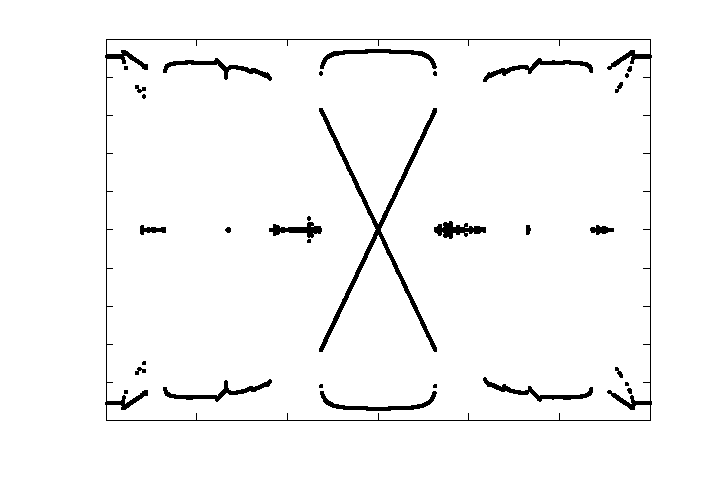
\includegraphics[width={324.00bp},height={216.00bp}]{images/FrequencyBifurcation}}%
    \gplfronttext
  \end{picture}%
\endgroup
}
    \caption{Bifurcation diagram of frequencies from the oscillating magnetic field $\Omega$ and the response frequencies on the dipole $\omega$, for the case with $\varepsilon = 0.5$.}
    \label{fig:bif05}
\end{figure}
\begin{figure*}
    \begin{subfigure}{\textwidth}
        % GNUPLOT: LaTeX picture with Postscript
\begingroup
  \makeatletter
  \providecommand\color[2][]{%
    \GenericError{(gnuplot) \space\space\space\@spaces}{%
      Package color not loaded in conjunction with
      terminal option `colourtext'%
    }{See the gnuplot documentation for explanation.%
    }{Either use 'blacktext' in gnuplot or load the package
      color.sty in LaTeX.}%
    \renewcommand\color[2][]{}%
  }%
  \providecommand\includegraphics[2][]{%
    \GenericError{(gnuplot) \space\space\space\@spaces}{%
      Package graphicx or graphics not loaded%
    }{See the gnuplot documentation for explanation.%
    }{The gnuplot epslatex terminal needs graphicx.sty or graphics.sty.}%
    \renewcommand\includegraphics[2][]{}%
  }%
  \providecommand\rotatebox[2]{#2}%
  \@ifundefined{ifGPcolor}{%
    \newif\ifGPcolor
    \GPcolortrue
  }{}%
  \@ifundefined{ifGPblacktext}{%
    \newif\ifGPblacktext
    \GPblacktexttrue
  }{}%
  % define a \g@addto@macro without @ in the name:
  \let\gplgaddtomacro\g@addto@macro
  % define empty templates for all commands taking text:
  \gdef\gplbacktext{}%
  \gdef\gplfronttext{}%
  \makeatother
  \ifGPblacktext
    % no textcolor at all
    \def\colorrgb#1{}%
    \def\colorgray#1{}%
  \else
    % gray or color?
    \ifGPcolor
      \def\colorrgb#1{\color[rgb]{#1}}%
      \def\colorgray#1{\color[gray]{#1}}%
      \expandafter\def\csname LTw\endcsname{\color{white}}%
      \expandafter\def\csname LTb\endcsname{\color{black}}%
      \expandafter\def\csname LTa\endcsname{\color{black}}%
      \expandafter\def\csname LT0\endcsname{\color[rgb]{1,0,0}}%
      \expandafter\def\csname LT1\endcsname{\color[rgb]{0,1,0}}%
      \expandafter\def\csname LT2\endcsname{\color[rgb]{0,0,1}}%
      \expandafter\def\csname LT3\endcsname{\color[rgb]{1,0,1}}%
      \expandafter\def\csname LT4\endcsname{\color[rgb]{0,1,1}}%
      \expandafter\def\csname LT5\endcsname{\color[rgb]{1,1,0}}%
      \expandafter\def\csname LT6\endcsname{\color[rgb]{0,0,0}}%
      \expandafter\def\csname LT7\endcsname{\color[rgb]{1,0.3,0}}%
      \expandafter\def\csname LT8\endcsname{\color[rgb]{0.5,0.5,0.5}}%
    \else
      % gray
      \def\colorrgb#1{\color{black}}%
      \def\colorgray#1{\color[gray]{#1}}%
      \expandafter\def\csname LTw\endcsname{\color{white}}%
      \expandafter\def\csname LTb\endcsname{\color{black}}%
      \expandafter\def\csname LTa\endcsname{\color{black}}%
      \expandafter\def\csname LT0\endcsname{\color{black}}%
      \expandafter\def\csname LT1\endcsname{\color{black}}%
      \expandafter\def\csname LT2\endcsname{\color{black}}%
      \expandafter\def\csname LT3\endcsname{\color{black}}%
      \expandafter\def\csname LT4\endcsname{\color{black}}%
      \expandafter\def\csname LT5\endcsname{\color{black}}%
      \expandafter\def\csname LT6\endcsname{\color{black}}%
      \expandafter\def\csname LT7\endcsname{\color{black}}%
      \expandafter\def\csname LT8\endcsname{\color{black}}%
    \fi
  \fi
    \setlength{\unitlength}{0.0500bp}%
    \ifx\gptboxheight\undefined%
      \newlength{\gptboxheight}%
      \newlength{\gptboxwidth}%
      \newsavebox{\gptboxtext}%
    \fi%
    \setlength{\fboxrule}{0.5pt}%
    \setlength{\fboxsep}{1pt}%
    \definecolor{tbcol}{rgb}{1,1,1}%
\begin{picture}(8640.00,2520.00)%
    \gplgaddtomacro\gplbacktext{%
      \csname LTb\endcsname%%
      \put(688,512){\makebox(0,0)[r]{\strut{}$-2$}}%
      \put(688,743){\makebox(0,0)[r]{\strut{}$-1.5$}}%
      \put(688,974){\makebox(0,0)[r]{\strut{}$-1$}}%
      \put(688,1205){\makebox(0,0)[r]{\strut{}$-0.5$}}%
      \put(688,1436){\makebox(0,0)[r]{\strut{}$0$}}%
      \put(688,1666){\makebox(0,0)[r]{\strut{}$0.5$}}%
      \put(688,1897){\makebox(0,0)[r]{\strut{}$1$}}%
      \put(688,2128){\makebox(0,0)[r]{\strut{}$1.5$}}%
      \put(688,2359){\makebox(0,0)[r]{\strut{}$2$}}%
      \put(784,352){\makebox(0,0){\strut{}$0$}}%
      \put(2676,352){\makebox(0,0){\strut{}$50$}}%
      \put(4568,352){\makebox(0,0){\strut{}$100$}}%
      \put(6459,352){\makebox(0,0){\strut{}$150$}}%
      \put(8351,352){\makebox(0,0){\strut{}$200$}}%
    }%
    \gplgaddtomacro\gplfronttext{%
      \csname LTb\endcsname%%
      \put(152,1435){\rotatebox{-270}{\makebox(0,0){\strut{}$\theta (t)$}}}%
      % \put(4567,112){\makebox(0,0){\strut{}Time}}%
    }%
    \gplbacktext
    \put(0,0){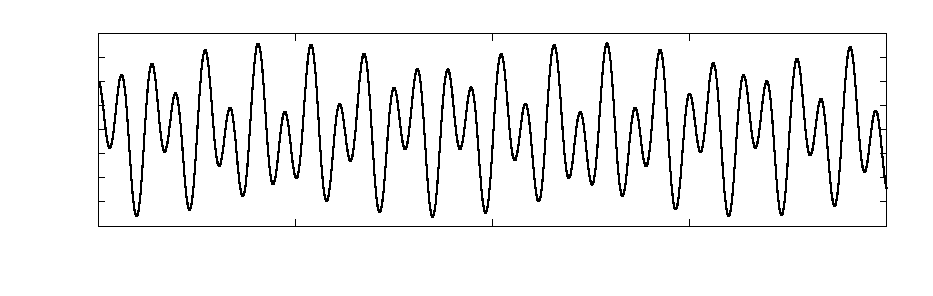
\includegraphics[width={432.00bp},height={126.00bp}]{images/omega05}}%
    \gplfronttext
  \end{picture}%
\endgroup

        \caption{Movement of the dipole with frequency of the external magnetic field being 0.5.}
        \label{fig:omega05}
    \end{subfigure}
    \begin{subfigure}{\textwidth}
        % GNUPLOT: LaTeX picture with Postscript
\begingroup
  \makeatletter
  \providecommand\color[2][]{%
    \GenericError{(gnuplot) \space\space\space\@spaces}{%
      Package color not loaded in conjunction with
      terminal option `colourtext'%
    }{See the gnuplot documentation for explanation.%
    }{Either use 'blacktext' in gnuplot or load the package
      color.sty in LaTeX.}%
    \renewcommand\color[2][]{}%
  }%
  \providecommand\includegraphics[2][]{%
    \GenericError{(gnuplot) \space\space\space\@spaces}{%
      Package graphicx or graphics not loaded%
    }{See the gnuplot documentation for explanation.%
    }{The gnuplot epslatex terminal needs graphicx.sty or graphics.sty.}%
    \renewcommand\includegraphics[2][]{}%
  }%
  \providecommand\rotatebox[2]{#2}%
  \@ifundefined{ifGPcolor}{%
    \newif\ifGPcolor
    \GPcolortrue
  }{}%
  \@ifundefined{ifGPblacktext}{%
    \newif\ifGPblacktext
    \GPblacktexttrue
  }{}%
  % define a \g@addto@macro without @ in the name:
  \let\gplgaddtomacro\g@addto@macro
  % define empty templates for all commands taking text:
  \gdef\gplbacktext{}%
  \gdef\gplfronttext{}%
  \makeatother
  \ifGPblacktext
    % no textcolor at all
    \def\colorrgb#1{}%
    \def\colorgray#1{}%
  \else
    % gray or color?
    \ifGPcolor
      \def\colorrgb#1{\color[rgb]{#1}}%
      \def\colorgray#1{\color[gray]{#1}}%
      \expandafter\def\csname LTw\endcsname{\color{white}}%
      \expandafter\def\csname LTb\endcsname{\color{black}}%
      \expandafter\def\csname LTa\endcsname{\color{black}}%
      \expandafter\def\csname LT0\endcsname{\color[rgb]{1,0,0}}%
      \expandafter\def\csname LT1\endcsname{\color[rgb]{0,1,0}}%
      \expandafter\def\csname LT2\endcsname{\color[rgb]{0,0,1}}%
      \expandafter\def\csname LT3\endcsname{\color[rgb]{1,0,1}}%
      \expandafter\def\csname LT4\endcsname{\color[rgb]{0,1,1}}%
      \expandafter\def\csname LT5\endcsname{\color[rgb]{1,1,0}}%
      \expandafter\def\csname LT6\endcsname{\color[rgb]{0,0,0}}%
      \expandafter\def\csname LT7\endcsname{\color[rgb]{1,0.3,0}}%
      \expandafter\def\csname LT8\endcsname{\color[rgb]{0.5,0.5,0.5}}%
    \else
      % gray
      \def\colorrgb#1{\color{black}}%
      \def\colorgray#1{\color[gray]{#1}}%
      \expandafter\def\csname LTw\endcsname{\color{white}}%
      \expandafter\def\csname LTb\endcsname{\color{black}}%
      \expandafter\def\csname LTa\endcsname{\color{black}}%
      \expandafter\def\csname LT0\endcsname{\color{black}}%
      \expandafter\def\csname LT1\endcsname{\color{black}}%
      \expandafter\def\csname LT2\endcsname{\color{black}}%
      \expandafter\def\csname LT3\endcsname{\color{black}}%
      \expandafter\def\csname LT4\endcsname{\color{black}}%
      \expandafter\def\csname LT5\endcsname{\color{black}}%
      \expandafter\def\csname LT6\endcsname{\color{black}}%
      \expandafter\def\csname LT7\endcsname{\color{black}}%
      \expandafter\def\csname LT8\endcsname{\color{black}}%
    \fi
  \fi
    \setlength{\unitlength}{0.0500bp}%
    \ifx\gptboxheight\undefined%
      \newlength{\gptboxheight}%
      \newlength{\gptboxwidth}%
      \newsavebox{\gptboxtext}%
    \fi%
    \setlength{\fboxrule}{0.5pt}%
    \setlength{\fboxsep}{1pt}%
    \definecolor{tbcol}{rgb}{1,1,1}%
\begin{picture}(8640.00,2520.00)%
    \gplgaddtomacro\gplbacktext{%
      \csname LTb\endcsname%%
      \put(592,512){\makebox(0,0)[r]{\strut{}$-70$}}%
      \put(592,743){\makebox(0,0)[r]{\strut{}$-60$}}%
      \put(592,974){\makebox(0,0)[r]{\strut{}$-50$}}%
      \put(592,1205){\makebox(0,0)[r]{\strut{}$-40$}}%
      \put(592,1436){\makebox(0,0)[r]{\strut{}$-30$}}%
      \put(592,1666){\makebox(0,0)[r]{\strut{}$-20$}}%
      \put(592,1897){\makebox(0,0)[r]{\strut{}$-10$}}%
      \put(592,2128){\makebox(0,0)[r]{\strut{}$0$}}%
      \put(592,2359){\makebox(0,0)[r]{\strut{}$10$}}%
      \put(784,352){\makebox(0,0){\strut{}$0$}}%
      \put(2676,352){\makebox(0,0){\strut{}$50$}}%
      \put(4568,352){\makebox(0,0){\strut{}$100$}}%
      \put(6459,352){\makebox(0,0){\strut{}$150$}}%
      \put(8351,352){\makebox(0,0){\strut{}$200$}}%
    }%
    \gplgaddtomacro\gplfronttext{%
      \csname LTb\endcsname%%
      \put(152,1435){\rotatebox{-270}{\makebox(0,0){\strut{}$\theta (t)$}}}%
      \put(4519,112){\makebox(0,0){\strut{}Time}}%
    }%
    \gplbacktext
    \put(0,0){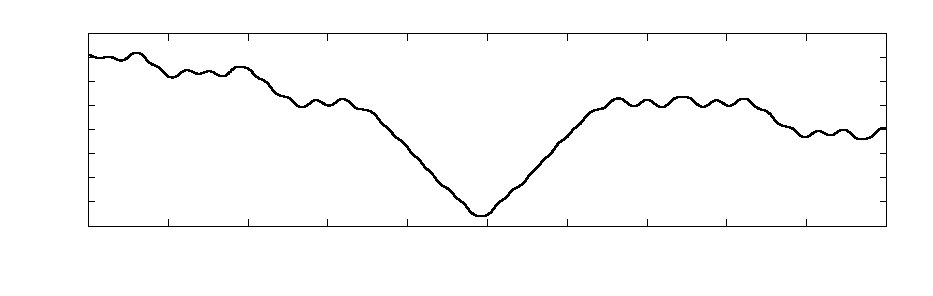
\includegraphics[width={432.00bp},height={126.00bp}]{images/omega075}}%
    \gplfronttext
  \end{picture}%
\endgroup

        \caption{Movement of the dipole with frequency of the external magnetic field being 0.75.}
        \label{fig:omega075}
    \end{subfigure}
    \begin{subfigure}{\textwidth}
        % GNUPLOT: LaTeX picture with Postscript
\begingroup
  \makeatletter
  \providecommand\color[2][]{%
    \GenericError{(gnuplot) \space\space\space\@spaces}{%
      Package color not loaded in conjunction with
      terminal option `colourtext'%
    }{See the gnuplot documentation for explanation.%
    }{Either use 'blacktext' in gnuplot or load the package
      color.sty in LaTeX.}%
    \renewcommand\color[2][]{}%
  }%
  \providecommand\includegraphics[2][]{%
    \GenericError{(gnuplot) \space\space\space\@spaces}{%
      Package graphicx or graphics not loaded%
    }{See the gnuplot documentation for explanation.%
    }{The gnuplot epslatex terminal needs graphicx.sty or graphics.sty.}%
    \renewcommand\includegraphics[2][]{}%
  }%
  \providecommand\rotatebox[2]{#2}%
  \@ifundefined{ifGPcolor}{%
    \newif\ifGPcolor
    \GPcolortrue
  }{}%
  \@ifundefined{ifGPblacktext}{%
    \newif\ifGPblacktext
    \GPblacktexttrue
  }{}%
  % define a \g@addto@macro without @ in the name:
  \let\gplgaddtomacro\g@addto@macro
  % define empty templates for all commands taking text:
  \gdef\gplbacktext{}%
  \gdef\gplfronttext{}%
  \makeatother
  \ifGPblacktext
    % no textcolor at all
    \def\colorrgb#1{}%
    \def\colorgray#1{}%
  \else
    % gray or color?
    \ifGPcolor
      \def\colorrgb#1{\color[rgb]{#1}}%
      \def\colorgray#1{\color[gray]{#1}}%
      \expandafter\def\csname LTw\endcsname{\color{white}}%
      \expandafter\def\csname LTb\endcsname{\color{black}}%
      \expandafter\def\csname LTa\endcsname{\color{black}}%
      \expandafter\def\csname LT0\endcsname{\color[rgb]{1,0,0}}%
      \expandafter\def\csname LT1\endcsname{\color[rgb]{0,1,0}}%
      \expandafter\def\csname LT2\endcsname{\color[rgb]{0,0,1}}%
      \expandafter\def\csname LT3\endcsname{\color[rgb]{1,0,1}}%
      \expandafter\def\csname LT4\endcsname{\color[rgb]{0,1,1}}%
      \expandafter\def\csname LT5\endcsname{\color[rgb]{1,1,0}}%
      \expandafter\def\csname LT6\endcsname{\color[rgb]{0,0,0}}%
      \expandafter\def\csname LT7\endcsname{\color[rgb]{1,0.3,0}}%
      \expandafter\def\csname LT8\endcsname{\color[rgb]{0.5,0.5,0.5}}%
    \else
      % gray
      \def\colorrgb#1{\color{black}}%
      \def\colorgray#1{\color[gray]{#1}}%
      \expandafter\def\csname LTw\endcsname{\color{white}}%
      \expandafter\def\csname LTb\endcsname{\color{black}}%
      \expandafter\def\csname LTa\endcsname{\color{black}}%
      \expandafter\def\csname LT0\endcsname{\color{black}}%
      \expandafter\def\csname LT1\endcsname{\color{black}}%
      \expandafter\def\csname LT2\endcsname{\color{black}}%
      \expandafter\def\csname LT3\endcsname{\color{black}}%
      \expandafter\def\csname LT4\endcsname{\color{black}}%
      \expandafter\def\csname LT5\endcsname{\color{black}}%
      \expandafter\def\csname LT6\endcsname{\color{black}}%
      \expandafter\def\csname LT7\endcsname{\color{black}}%
      \expandafter\def\csname LT8\endcsname{\color{black}}%
    \fi
  \fi
    \setlength{\unitlength}{0.0500bp}%
    \ifx\gptboxheight\undefined%
      \newlength{\gptboxheight}%
      \newlength{\gptboxwidth}%
      \newsavebox{\gptboxtext}%
    \fi%
    \setlength{\fboxrule}{0.5pt}%
    \setlength{\fboxsep}{1pt}%
    \definecolor{tbcol}{rgb}{1,1,1}%
\begin{picture}(8640.00,2520.00)%
    \gplgaddtomacro\gplbacktext{%
      \csname LTb\endcsname%%
      \put(688,512){\makebox(0,0)[r]{\strut{}$-1.5$}}%
      \put(688,820){\makebox(0,0)[r]{\strut{}$-1$}}%
      \put(688,1128){\makebox(0,0)[r]{\strut{}$-0.5$}}%
      \put(688,1436){\makebox(0,0)[r]{\strut{}$0$}}%
      \put(688,1743){\makebox(0,0)[r]{\strut{}$0.5$}}%
      \put(688,2051){\makebox(0,0)[r]{\strut{}$1$}}%
      \put(688,2359){\makebox(0,0)[r]{\strut{}$1.5$}}%
      \put(784,352){\makebox(0,0){\strut{}$0$}}%
      \put(2676,352){\makebox(0,0){\strut{}$50$}}%
      \put(4568,352){\makebox(0,0){\strut{}$100$}}%
      \put(6459,352){\makebox(0,0){\strut{}$150$}}%
      \put(8351,352){\makebox(0,0){\strut{}$200$}}%
    }%
    \gplgaddtomacro\gplfronttext{%
      \csname LTb\endcsname%%
      \put(152,1435){\rotatebox{-270}{\makebox(0,0){\strut{}$\theta (t)$}}}%
      % \put(4567,112){\makebox(0,0){\strut{}Time}}%
    }%
    \gplbacktext
    \put(0,0){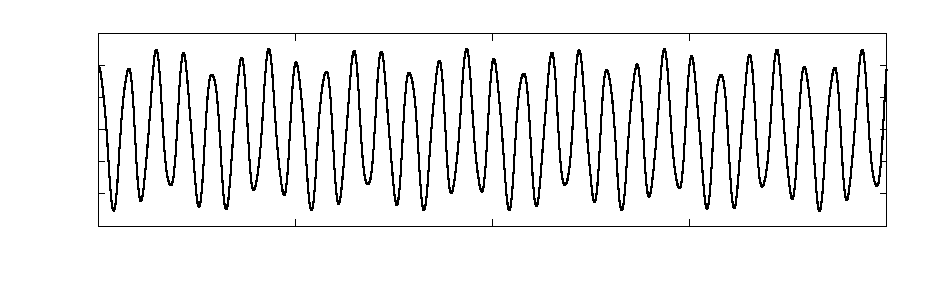
\includegraphics[width={432.00bp},height={126.00bp}]{images/omega20}}%
    \gplfronttext
  \end{picture}%
\endgroup

        \caption{Movement of the dipole with frequency of the external magnetic field being 2.0.}
        \label{fig:omega20}
    \end{subfigure}
    \caption{Movement of the dipole for different frequencies of the magnetic field. Using $\varepsilon = 0.5$}
\end{figure*}
